\documentclass[../main.tex]{subfiles}
\graphicspath{{\subfix{../imgs/}}}
\begin{document}

% OJO
\chapter{Aplicaciones con robots aéreos} \label{cap:aplic}
Este capítulo recoge las dos aplicaciones desarrolladas sobre la infraestructura presentada. El objetivo principal de las mismas es ilustrar el uso de la infraestructura, incluyendo el manejo de visión con Aprendizaje profundo y el control en velocidad que permite validar su correcto funcionamiento. En diferentes secciones, se muestran los dos experimentos desarrollados, \emph{sigue-color} y \emph{sigue-persona}. Sobre ambos se explican los diseños ideados, su implementación y los resultados obtenidos con las diferentes plataformas.

\section{Aplicación Sigue Color} \label{section:aplic-color}
La aplicación \emph{sigue-color} consiste en el seguimiento por parte de la aeronave de un elemento de un color llamativo. La aplicación se ha probado sobre dos aeronaves, el dron simulado y el Tello real. Las balizas cromáticas, o elementos a seguir, utilizadas para cada uno de los experimentos se muestran en la Figura \ref{fig:balizas}. Sobre la baliza simulada se han desarrollado varios \emph{plugins} de Gazebo para darle movimiento al modelo, bien sea con una trayectoria predeterminada o teleoperando desde teclado al objeto.

\begin{figure}[ht]
 	\ffigbox[\FBwidth]{
     	\begin{subfigure}{0.45\textwidth}
            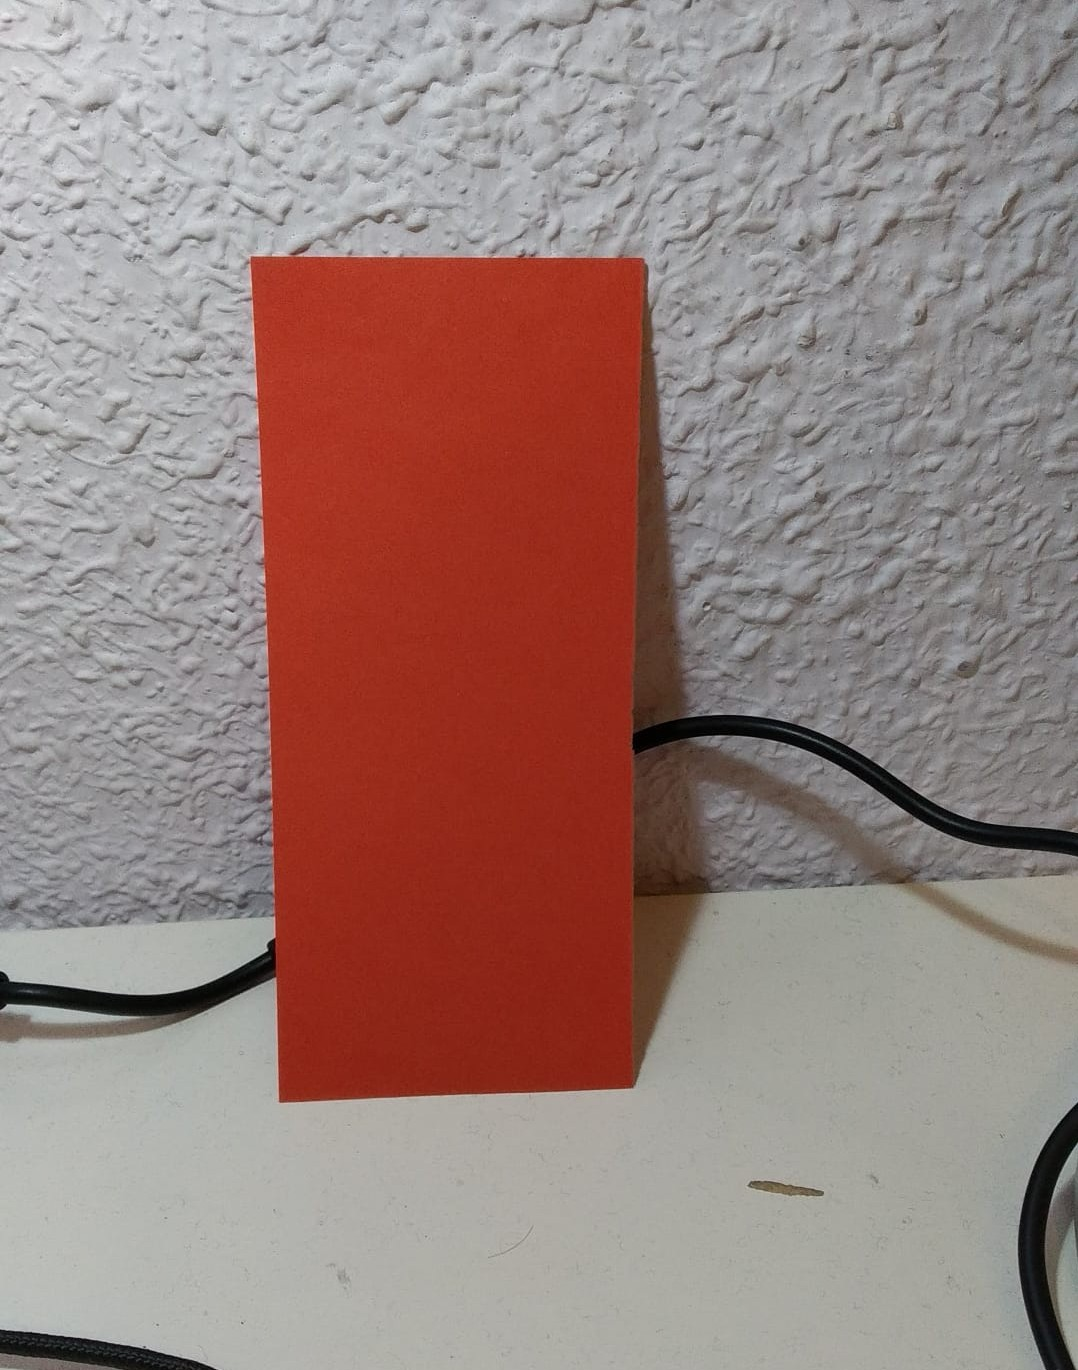
\includegraphics[height=5cm]{05/in.jpeg}
            \caption[Baliza real]{Baliza real.}
        \end{subfigure}
        \begin{subfigure}{0.45\textwidth}
            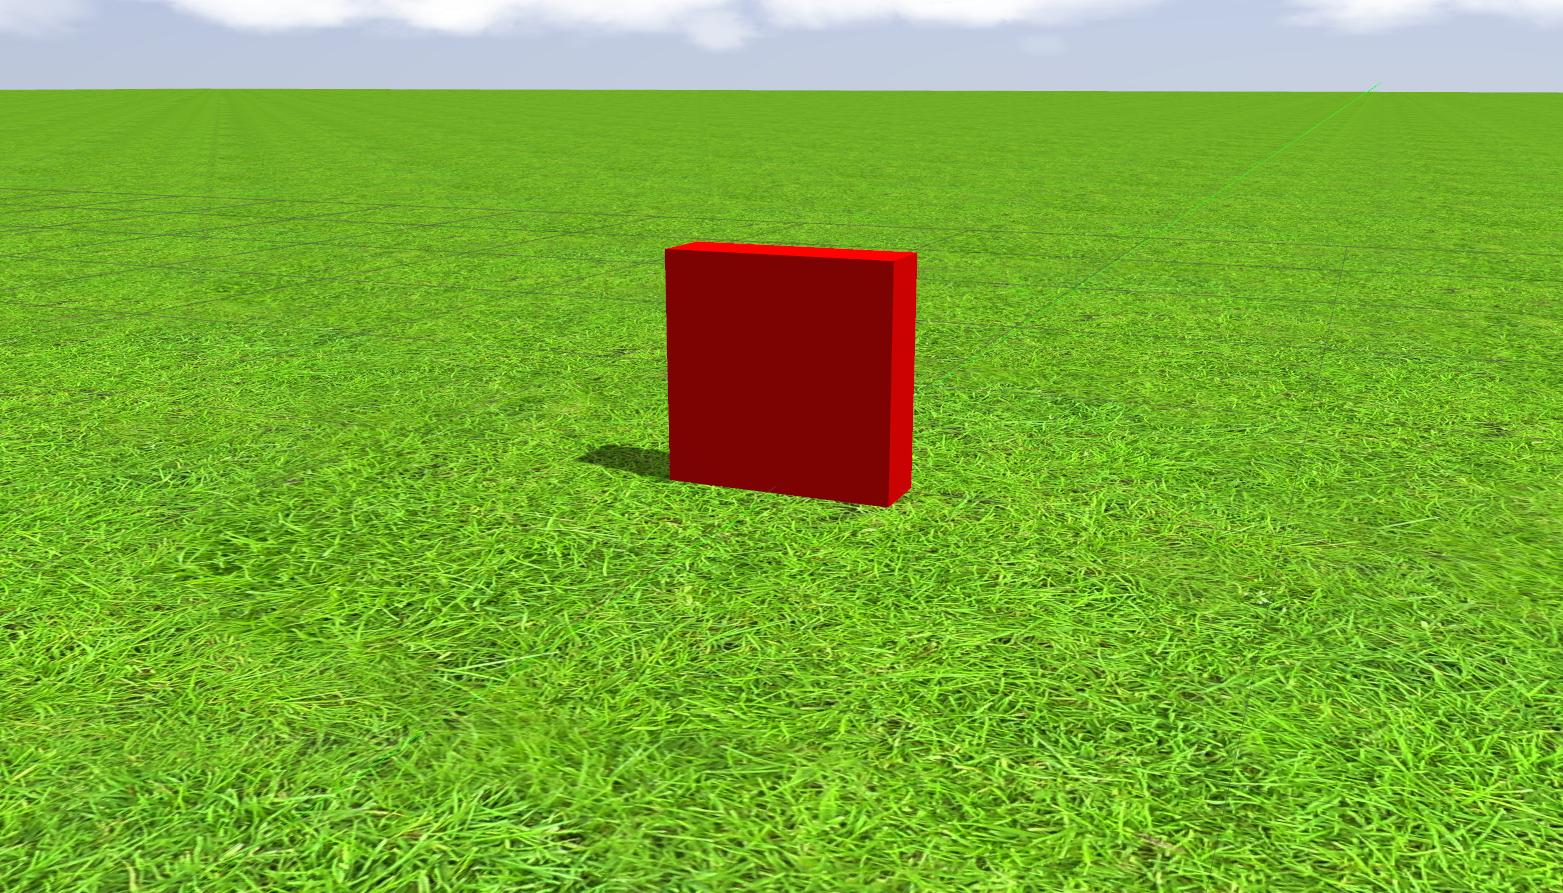
\includegraphics[height=4.25cm]{05/target.jpg}
            \caption[Baliza simulada]{Baliza simulada.}
        \end{subfigure}
 	}{
 	    \caption[Balizas utilizadas en \emph{sigue-color}]{Balizas utilizadas en \emph{sigue-color}.}
 	    \label{fig:balizas}
 	}
\end{figure}

La infraestructura permite compartir el mismo código fuente para ambas aeronaves, la real y la simulada. Sin embargo, las características de las aeronaves son muy diferentes. Utilizar la misma lógica para ambos drones es posible gracias a que la aplicación utiliza archivos de configuración donde se guardan ciertos parámetros intrínsecos a la aeronave. La Figura \ref{fig:esq-sc} muestra la estructura de la aplicación. \\
Estos ficheros de configuración guardan datos que permiten ajustar el código genérico a una aeronave concreta. Durante el lanzamiento de los procesos, los datos se cargan como parámetros de ROS, donde \emph{DroneWrapper} y \emph{sigue-color} pueden acceder fácilmente. En las sucesivas secciones se explicarán con más detalle los parámetros que contienen los archivos de configuración.

\begin{figure}[!ht]
 	\ffigbox[\FBwidth] {
 	    \caption[Estructura de \emph{sigue-color}]{Estructura de \emph{sigue-color}.}
        \label{fig:esq-sc}
    }
 	{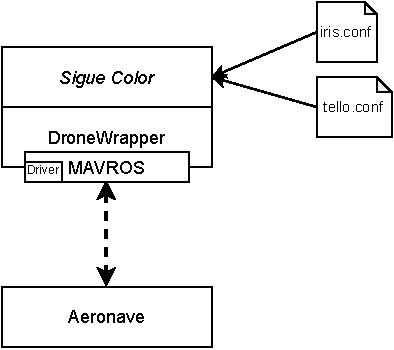
\includegraphics[width=0.5\textwidth]{05/follow-color.pdf}}
\end{figure}

\subsection*{Diseño}
El diseño de la aplicación del robot aéreo consiste en dos partes, la percepción y el control. La percepción se encarga de detectar visualmente el objeto a seguir, mientras que el control envía los comandos de movimiento a la aeronave para lograr seguir al objeto. La Figura \ref{fig:esq-sc-2} representa dicho diseño en un esquema de bloques.

\begin{figure}[!ht]
 	\ffigbox[\FBwidth] {
 	    \caption[Bloques presentes en \emph{sigue-color}]{Bloques presentes en \emph{sigue-color}.}
        \label{fig:esq-sc-2}
    }
 	{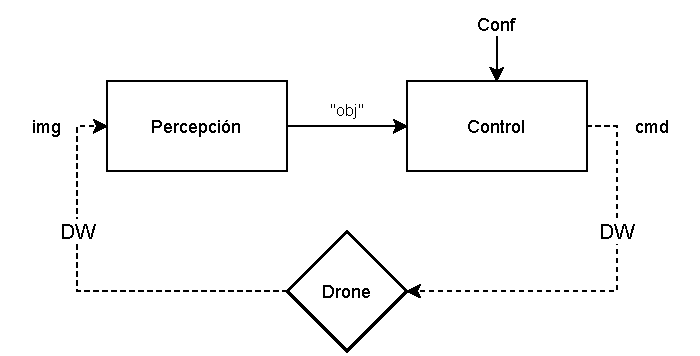
\includegraphics[width=0.9\textwidth]{05/fc-esquema.pdf}}
\end{figure}

El comportamiento de la aeronave se describe en el Código \ref{lst:fc-pseudo}. Tras el despegue, se inicia un bucle iterativo infinito donde se realizan las tareas de percepción y control. La percepción consiste en un filtrado por color de la imagen obtenida por la cámara del dron. Cuando se detecta algo en la percepción entra en acción el control. El control consta de tres controladores PID que calculan las velocidades comandadas a la aeronave. Si el filtrado de percepción no obtiene ninguna salida, la aeronave realiza un algoritmo de búsqueda hasta que encuentre un nuevo objeto al cual seguir. Este algoritmo de búsqueda consiste en dar vueltas sobre si mismo a una velocidad constante.

\lstinputlisting[caption={Pseudo-código de \emph{sigue-color}}, language=python, captionpos=b, label={lst:fc-pseudo}]{code/fc-pseudo.txt}

\subsection*{Percepción}
La percepción es un filtrado por color de la imagen mediante técnicas clásicas. El filtrado se realiza gracias a la biblioteca de visión por ordenador OpenCV. A lo largo de la explicación, se harán referencia a diferentes métodos de la biblioteca que se utilizan en la aplicación.

El filtrado se realiza, en general, en el espectro HSV (\emph{Hue-Saturation-Value}, o Tono-Saturación-Brillo) en vez de en el espectro RGB (\emph{Red-Green-Blue}, o Rojo-Verde-Azul). Esto es debido a que el espectro HSV representa en un solo valor el tono del color (\emph{Hue} o Tono), mientras que el espectro RGB necesita tres campos para representar el tono y es mucho más frágil frente a cambios de iluminación en la escena, lo que dificulta el diseño del filtro.

El diseño del filtrado por color se compone de cuatro etapas:
\begin{enumerate}
    \item \textbf{Desenfoque gaussiano.} Desenfoque sobre imagen a color (RGB) para eliminar píxeles espúreos mediante \lstinline{cv2.GaussianBlur()} y transformación a espacio HSV.
    \item \textbf{Máscara HSV.} Máscara sobre espacio HSV mediante \lstinline{cv2.inRange()}, combinación bit a bit de imagen y máscara (\lstinline{cv2.bitwise_and()}) y conversión a imagen en escala de grises.
    \item \textbf{Umbralización.} Umbral de nivel fijo, y con valor $150$, sobre imagen en escala de grises \lstinline{cv2.threshold()}.
    \item \textbf{Segmentación.} Agrupación por contornos sobre imagen en blanco y negro para la detección de objetos (\lstinline{cv2.findContours()}).
\end{enumerate}

La máscara aplicada es, por la naturaleza del espacio HSV, una combinación de dos máscaras. Dicha combinación, es la suma de ambas máscaras: \lstinline{mask = mask1 + mask2}. Esto ocurre debido a la discontinuidad angular en el tono, ya que valores de tono $H=1$ o $H=359$ son valores cromáticamente similares aunque numéricamente sean muy distintos. La Tabla \ref{tab:sc-mask} refleja los valores seleccionados para la máscara.

\begin{figure}[!ht]
 	\ffigbox[\FBwidth] {
 	    \caption[Máscara del filtro de color]{Máscara del filtro de color.}
        \label{fig:esq-mask}
    }
 	{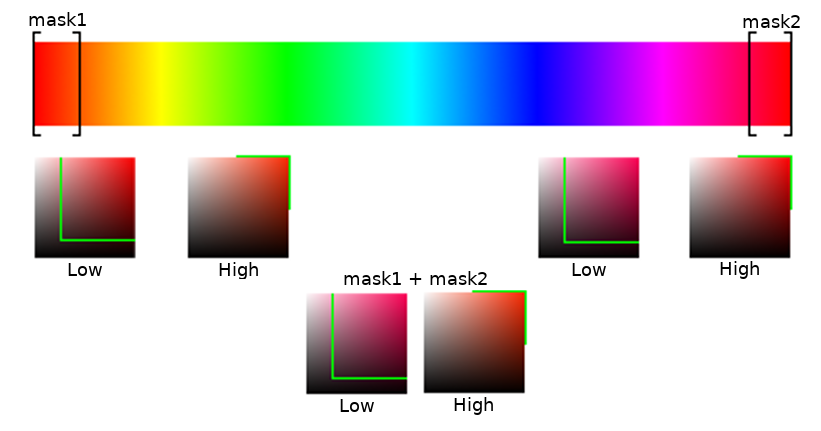
\includegraphics[width=\textwidth]{05/color_filter.png}}
\end{figure}

\begin{table}[H]
	\ttabbox[\FBwidth]
	{\caption{Máscaras HSV.} \label{tab:sc-mask}}
	{\begin{tabular}{|c|c|c|c|c|c|c|}
		\hline
		\multirow{2}{*}{\textbf{Máscara}} & \multicolumn{3}{c|}{\textbf{Mínimo}} & \multicolumn{3}{c|}{\textbf{Máximo}} \\
		\cline{2-7}
        & \textbf{H} & \textbf{S} & \textbf{V} & \textbf{H} & \textbf{S} & \textbf{V} \\
		\hline
		\lstinline{mask1} & 0 & 70 & 50 & 10 & 255 & 255 \\
        \hline
        \lstinline{mask2} & 340 & 70 & 50 & 359 & 255 & 255 \\
		\hline
		\multicolumn{7}{l}{Fuente: Elaboración propia}
	\end{tabular}}
\end{table}

Dicho valores pueden resultar algo confusos con su representación numérica. Para facilitar su comprensión, se ilustra en la Figura \ref{fig:esq-mask} una representación gráfica de las máscaras usadas.

\begin{figure}[!ht]
 	\ffigbox[\FBwidth] {
 	    \caption[Esquema de la percepción]{Esquema de la percepción.}
        \label{fig:esq-perc-sc}
    }
 	{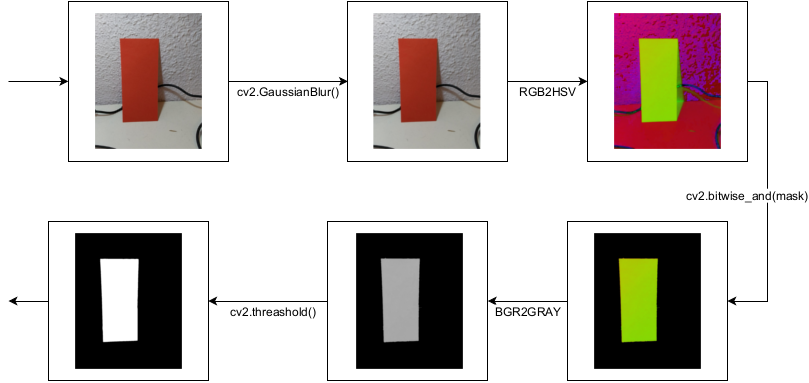
\includegraphics[width=\textwidth]{05/fc-percp.png}}
\end{figure}

El proceso seguido durante el bloque de percepción se muestra en la Figura \ref{fig:esq-perc-sc}. Como se puede observar en la figura, el filtrado da por resultado una imagen binaria (en blanco y negro). Sobre esta imagen, los píxeles detectados (en blanco) se agrupan por contornos en objetos \lstinline{cv2.findContours()}. En caso de detectar varios objetos, el objeto a seguir es aquel con el área más grande. Así pues, la Figura \ref{fig:filtrado} muestra la salida según una entrada concreta.

\begin{figure}[ht]
 	\ffigbox[\FBwidth]{
     	\begin{subfigure}{0.45\textwidth}
            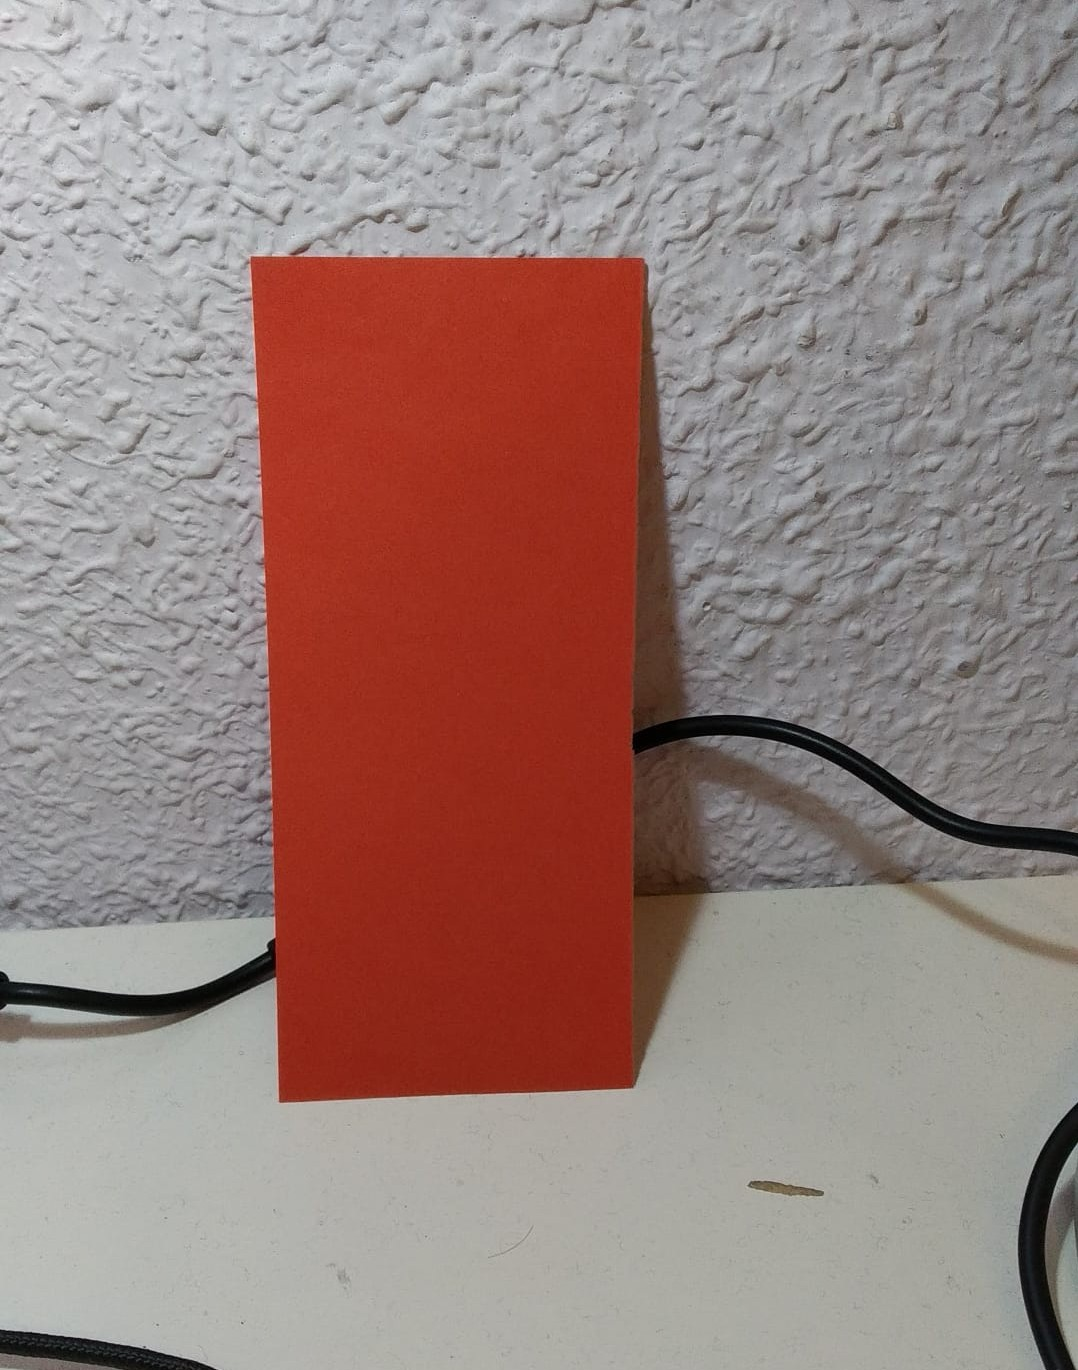
\includegraphics[width=0.9\linewidth]{05/in.jpeg}
            \caption{Entrada.}
        \end{subfigure}
        \begin{subfigure}{0.45\textwidth}
            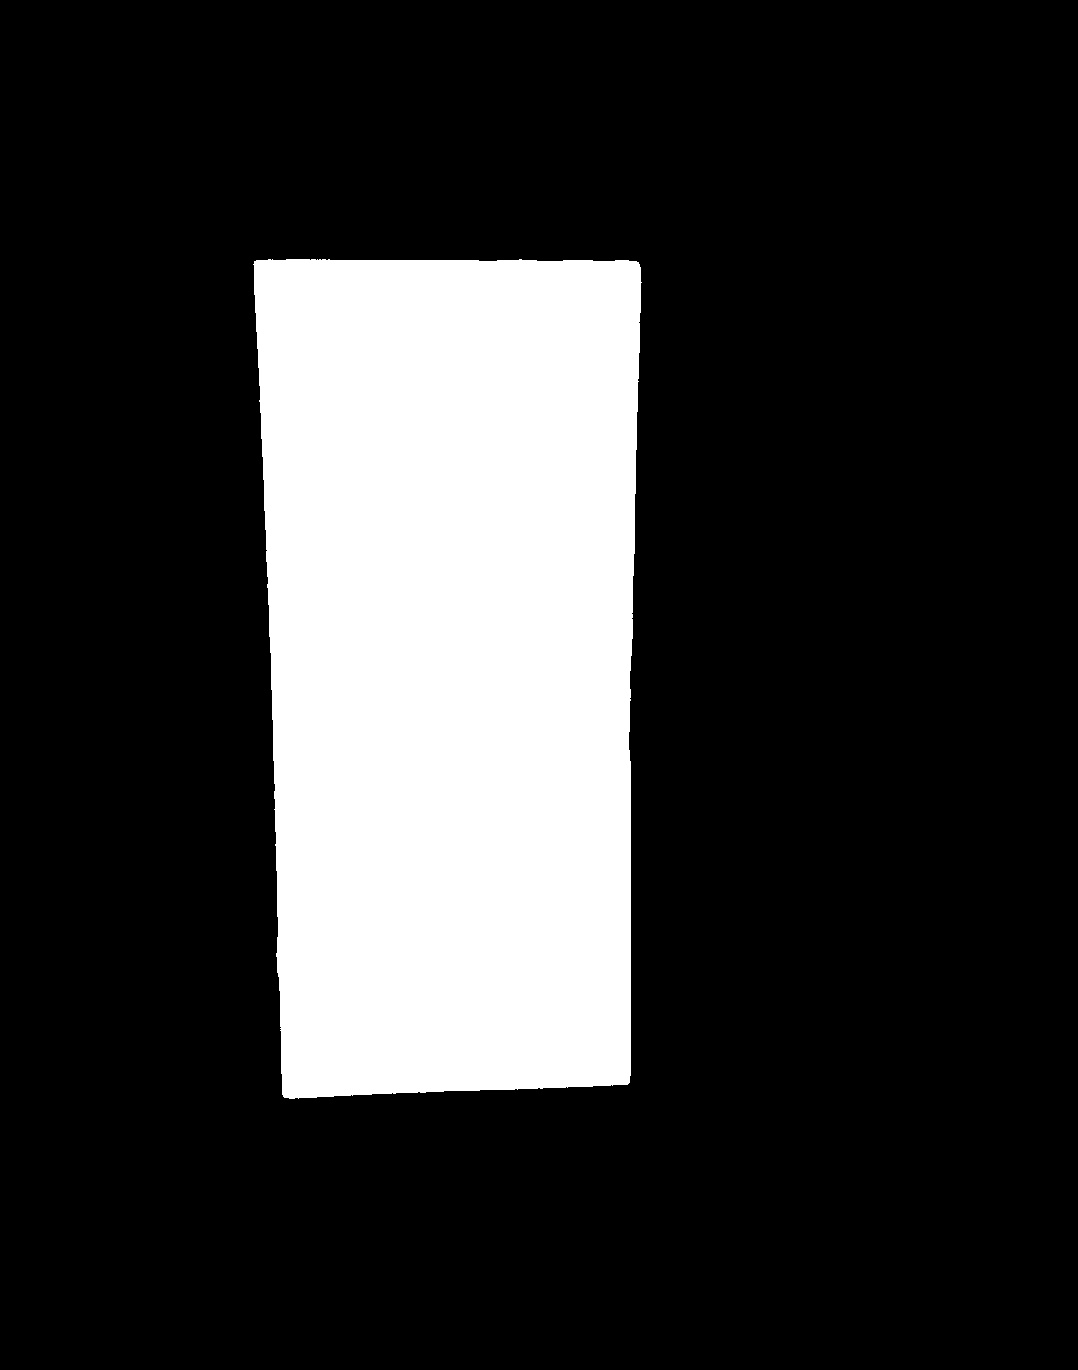
\includegraphics[width=0.9\linewidth]{05/out.jpg}
            \caption{Salida.}
        \end{subfigure}
 	}{
 	    \caption[Entrada y salida del filtrado]{Entrada y salida del filtrado.}
 	    \label{fig:filtrado}
 	}
\end{figure}

\subsection*{Control}
El bloque de control se ejecuta siempre con una entrada única, el objeto a seguir. Sobre este objeto se extraen propiedades como la posición sobre la imagen o el radio del mínimo círculo envolvente al contorno. Dichos valores se utilizan para calcular los errores o entradas de los controladores, y cuya salida son las \textit{velocidades} a comandar a la aeronave. La Figura \ref{fig:esq-control-sc} representa un esquema del bloque de control.

\begin{figure}[!ht]
 	\ffigbox[\FBwidth] {
 	    \caption[Esquema de control en \emph{sigue-color}]{Esquema de control en \emph{sigue-color}.}
        \label{fig:esq-control-sc}
    }
 	{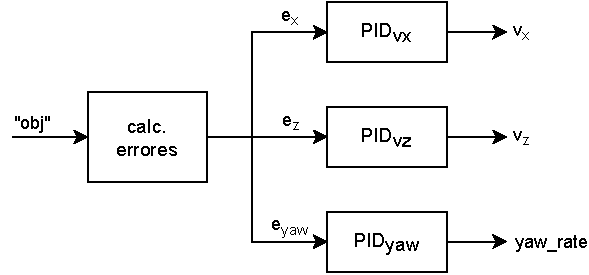
\includegraphics[width=0.65\textwidth]{05/fc-control.pdf}}
\end{figure}

En concreto son tres los controladores PID usados, uno que controla el avance (\lstinline{vx}), uno que controla la altura (\lstinline{vz}) y uno que controla el ángulo de guiñada (\lstinline{yaw_rate}). Las entradas para los controladores se calculan según las siguientes fórmulas:

\begin{align}
    e_x = & \frac{radio - target\_radio}{target\_radio} \label{eq:ex} \\
    e_z = & c_y - obj_y \label{eq:ez} \\
    e_{yaw} = & c_x - obj_x \label{eq:eyaw}
\end{align}

El control en altura y en guiñada (Ec. \ref{eq:ez} y Ec. \ref{eq:eyaw}) se realiza según la posición del centroide del objeto filtrado respecto del centro de la imagen (ver Fig. \ref{fig:sc-resp}). El control en avance (Ec. \ref{eq:ex}) es algo más complejo, pues utiliza la diferencia normalizada del radio del mínimo círculo envolvente al contorno y un radio de referencia ($target\_radio = 10$). De tal forma que, cuanto más pequeño sea el objeto en la imagen, más rápidamente avanzará el dron, hasta que el radio observado vuelve a estar cercano al de referencia. Dicho radio de referencia está relacionado con una distancia al objeto de aproximadamente 5 metros.

\begin{figure}[!ht]
 	\ffigbox[\FBwidth] {
 	    \caption{Respuesta del bloque de control en \emph{sigue-color}.}
        \label{fig:sc-resp}
    }
 	{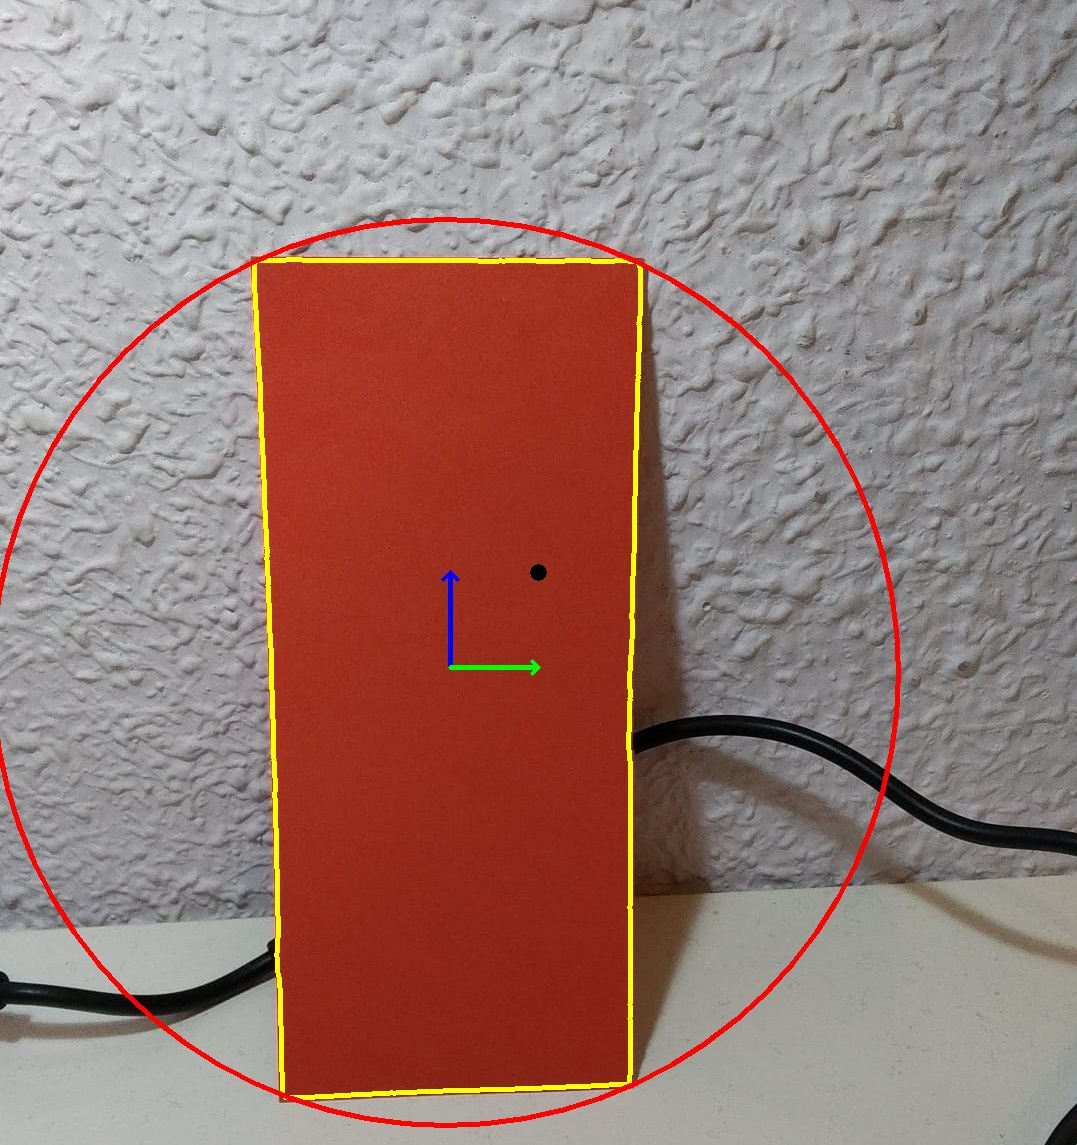
\includegraphics[width=0.65\textwidth]{05/error.jpg}}
\end{figure}

La Figura \ref{fig:sc-resp} muestra la respuesta dada por el bloque de control a una entrada cualquiera. Las flechas indican la dirección que tomará el dron para corregir el error existente, llevando el centro del objeto detectado hacia el centro de la imagen (punto negro). También se puede observar en la figura el contorno del objeto filtrado junto al círculo mínimo envolvente al contorno.

Los errores obtenidos son la alimentación de los controladores que tratan de reducir a cero estos valores con su respuesta, que son directamente los comandos de velocidad que se envían al dron. \\
La respuesta del controlador depende de las constantes del mismo ($k_P$, $k_I$, $k_D$). Dado que el control del dron depende de sus características intrínsecas concretas para ese modelo, las constantes de los controladores forman parte de los parámetros de los ficheros de configuración (ver Cód. \ref{lst:tello-conf}).

\lstinputlisting[caption={Fichero de configuración de la aeronave Tello}, language=python, captionpos=b, label={lst:tello-conf}]{code/tello.conf}

Las constantes de los controladores se han calculado de forma experimental para ambas aeronaves. El ajuste final de los valores se muestran en la Tabla \ref{tab:pid}.

\begin{table}[H]
	\ttabbox[\FBwidth]
	{\caption{Controladores PID y sus constantes.} \label{tab:pid}}
	{\begin{tabular}{|c|c|c|c|c|c|c|}
		\hline
		\multirow{2}{*}{\textbf{Controlador}} & \multicolumn{3}{c|}{\textbf{Iris}} & \multicolumn{3}{c|}{\textbf{Tello}} \\
		\cline{2-7}
        & \textbf{$k_P$} & \textbf{$k_I$} & \textbf{$k_D$} & \textbf{$k_P$} & \textbf{$k_I$} & \textbf{$k_D$} \\
		\hline
		\lstinline{vx} & 0.05 & 0.0 & 0.001 & 0.02 & 0.0 & 0.0002 \\
        \hline
        \lstinline{vy} & 0.0 & 0.0 & 0.0 & 0.0 & 0.0 & 0.0 \\
        \hline
		\lstinline{vz} & -0.02 & 0.0 & 0.001 & -0.0015 & 0.0 & 0.0 \\
        \hline
		\lstinline{yaw_rate} & -0.005 & 0.0 & 0.001 & 0.002 & 0.0 & 0.0001 \\
        \hline
		\multicolumn{7}{l}{Fuente: Elaboración propia}
	\end{tabular}}
\end{table}

\subsection*{Resultados}
Los resultados obtenidos se presentan en forma de distintas pruebas o experimentos. En general, se parte de un caso sencillo y se incrementa la dificultad del mismo en los sucesivos casos. Para el \emph{sigue-color}, se ha partido de experimento simple con el objeto a seguir estático y en simulación (ver Figura \ref{fig:sc-static}).

\begin{figure}[!ht]
 	\ffigbox[\FBwidth] {
 	    \caption{Experimento \emph{sigue-color} con modelo estático.}
        \label{fig:sc-static}
    }
 	{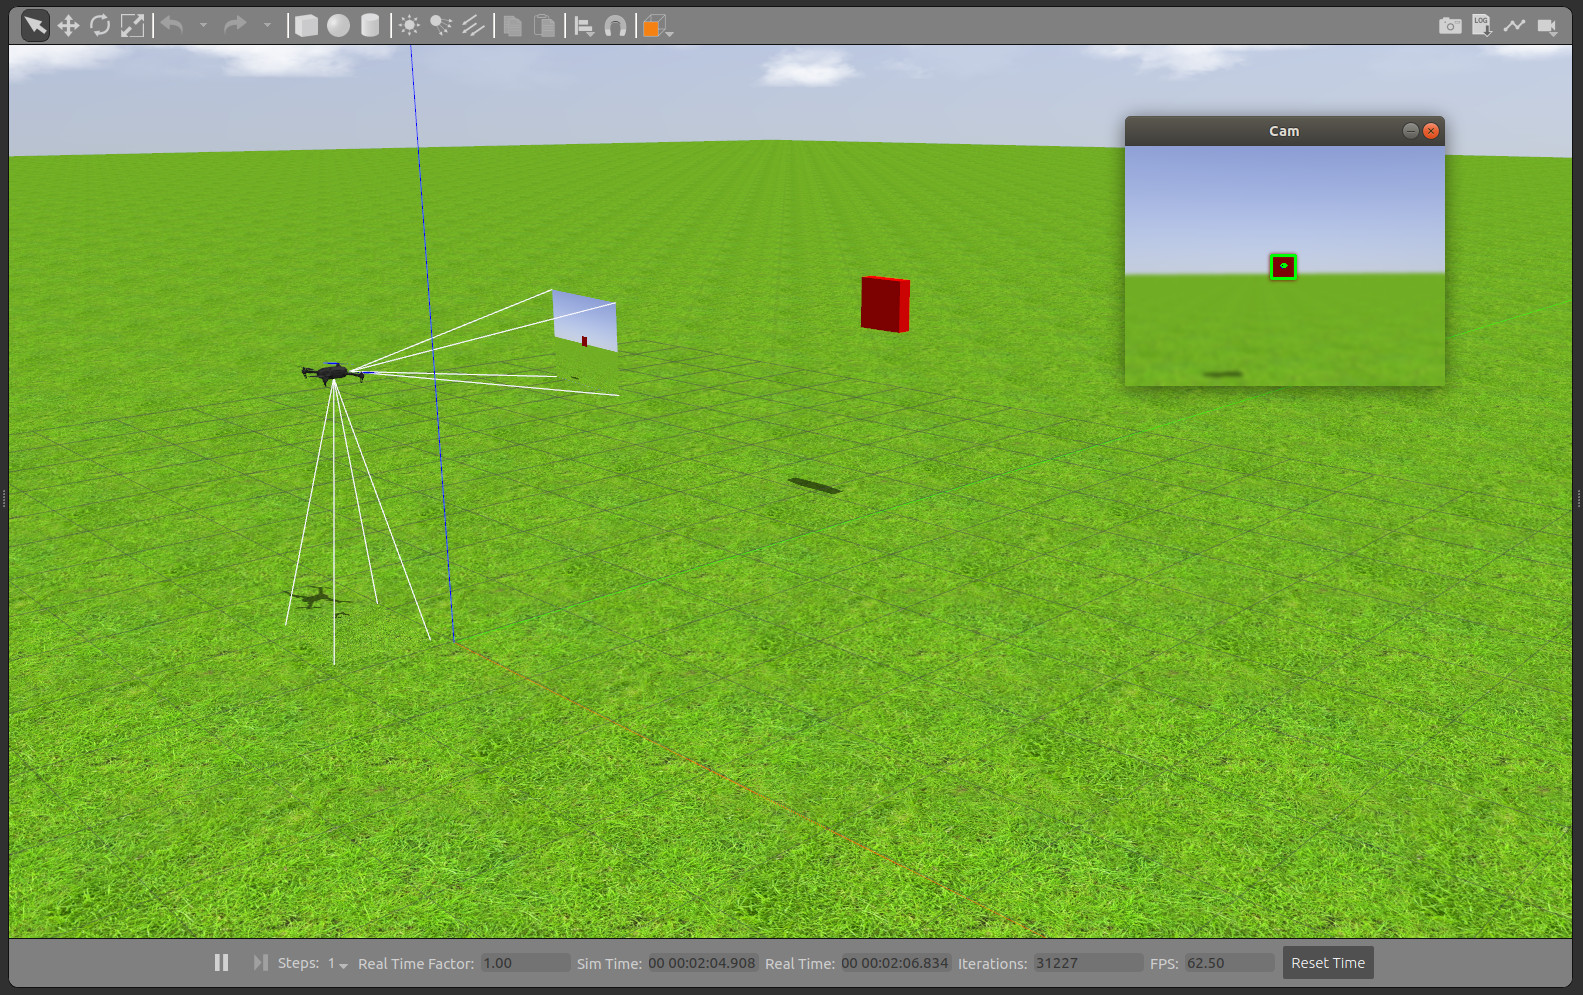
\includegraphics[width=0.85\textwidth]{05/static-fc.jpg}}
\end{figure}

\newpage
En segundo lugar, se ha probado la aplicación con un objeto en movimiento, primero moviendo el objeto manualmente a través de la herramienta de teleoperación desarrollada y con movimientos suaves. A continuación, se ha probado con un objeto con movimiento automático y acciones más bruscas y veloces que en el caso anterior.

Tras superar con éxito las pruebas en simulado, la aplicación se ha probado sobre el dron real Tello. De forma similar, los experimentos realizados han ido incrementando en dificultad hasta obtener un caso en movimiento con acciones rápidas y cambios bruscos.

Los diferentes experimentos están disponibles para su visualización en una lista de reproducción\footnote{\url{https://youtube.com/playlist?list=PL2ebURGAzRwusKLBYPJUkfZJ5SHudh6Z_}} que recoge los vídeos con cada uno de los experimentos (ver Fig. \ref{fig:yt-fc}).

\begin{figure}[!ht]
 	\ffigbox[\FBwidth] {
 	    \caption{Lista de reproducción \emph{sigue-color}.}
        \label{fig:yt-fc}
    }
 	{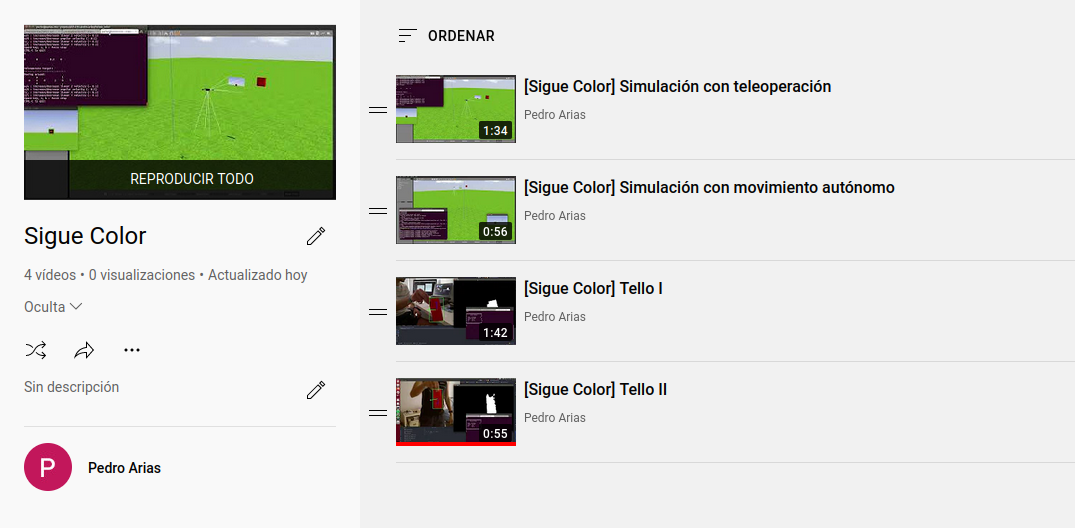
\includegraphics[width=0.9\textwidth]{05/yt-sigue-color.png}}
\end{figure}

%%%%%%
%%%%%%%%
%%%%%%%%%%
\newpage

\section{Aplicación Sigue Persona} \label{section:aplic-pers}
La aplicación \emph{sigue-persona} consiste en seguir a una persona con la aeronave. Existen diversos antecedentes de aplicaciones similares, como la desarrollada por Nacho Condés \cite{tfm-nacho, condes2020embedded} para robots terrestres. El experimento se ha realizado sobre las tres aeronaves disponibles, el dron simulado, el Tello y el PX4 de construcción propia. Para la simulación se ha utilizado un modelo perteneciente a la base de datos de \emph{Ignition Robotics} \cite{IgnitionFuel-OpenRobotics-Standing-person}. Sobre el modelo se han diseñado varios \emph{plugins} para dar movimiento a la persona. La Figura \ref{fig:persona} muestra el modelo utilizado.

\begin{figure}[ht]
 	\ffigbox[\FBwidth]{
     	\begin{subfigure}{0.45\textwidth}
            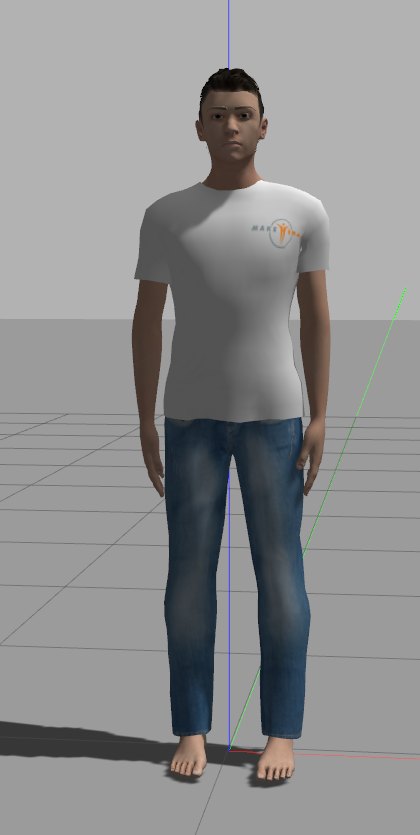
\includegraphics[height=6cm]{05/person1.png}
            \caption{Cuerpo entero.}
        \end{subfigure}
        \begin{subfigure}{0.45\textwidth}
            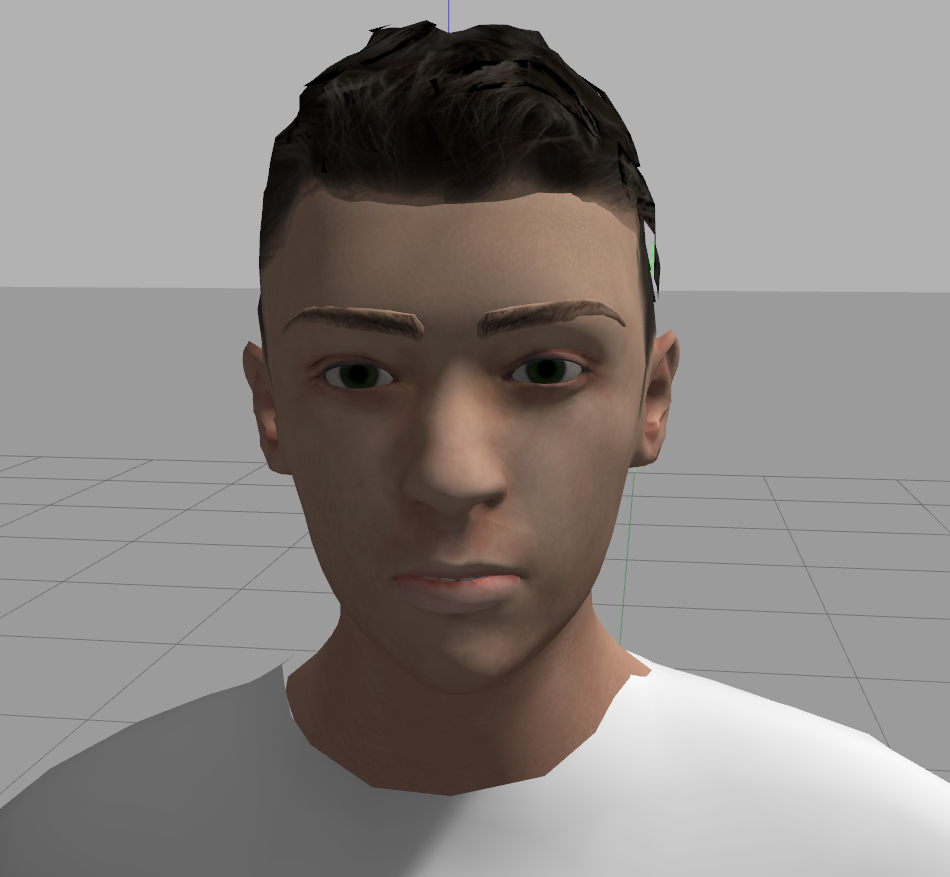
\includegraphics[height=6cm]{05/person2.png}
            \caption{Cara.}
        \end{subfigure}
 	}{
 	    \caption[Modelo de persona en el simulador Gazebo]{Modelo de persona en el simulador Gazebo \cite{IgnitionFuel-OpenRobotics-Standing-person}.}
 	    \label{fig:persona}
 	}
\end{figure}

La aplicación sigue el mismo diseño que el experimento anterior. La infraestructura pensada permite utilizar el mismo código fuente con distintos archivos de configuración. Así pues, el cuerpo de la aplicación es el mismo para las tres aeronaves. La Figura \ref{fig:esq-fp} muestra la estructura de la aplicación \emph{sigue-persona}.

\begin{figure}[!ht]
 	\ffigbox[\FBwidth] {
 	    \caption{Estructura de \emph{sigue-persona}}
        \label{fig:esq-fp}
    }
 	{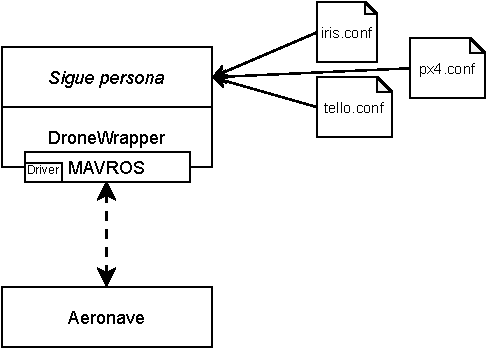
\includegraphics[width=0.65\textwidth]{05/follow-person.pdf}}
\end{figure}

\subsection*{Diseño}
El diseño es idéntico al ideado para el experimento anterior. La aplicación se compone de dos bloques, la percepción y el control. La percepción se encarga de detectar a la persona a seguir, mientras que el control se encarga de comandar a la aeronave. El esquema de bloques seguido se muestra en la Figura \ref{fig:esq-sp-2}.

\begin{figure}[!ht]
 	\ffigbox[\FBwidth] {
 	    \caption[Bloques presentes en \emph{sigue-persona}]{Bloques presentes en \emph{sigue-persona}.}
        \label{fig:esq-sp-2}
    }
 	{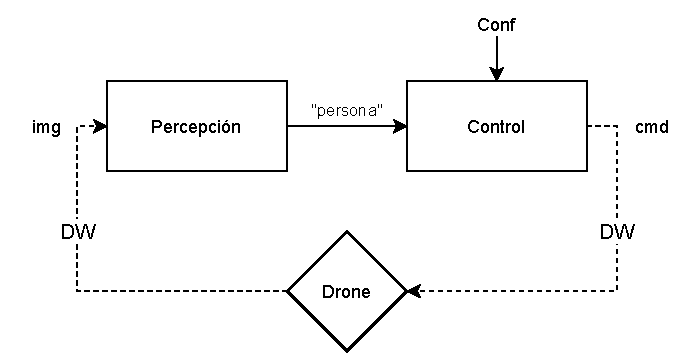
\includegraphics[width=0.8\textwidth]{05/fp-bloques.pdf}}
\end{figure}

Es importante destacar que la percepción es diferente entre las dos aplicaciones, detectar un objeto de color no conlleva la misma dificultad que detectar una persona, mientras que el control es idéntico entre ambas aplicaciones. Por tanto, el comportamiento de la aeronave (ver Cód. \ref{lst:fp-pseudo}) no es muy diferente entre aplicaciones.

\lstinputlisting[caption={Pseudo-código de \emph{sigue-persona}}, language=python, captionpos=b, label={lst:fp-pseudo}]{code/fp-pseudo.txt}

\subsection*{Percepción}
La percepción consta de dos partes, la detección robusta de la persona y la identificación de la misma. La detección se realiza mediante aprendizaje profundo, mientras que la identificación se consigue gracias a un seguimiento espacio-temporal con memoria finita de la detección.


La detección consiste en una red neuronal profunda, en concreto la red YOLOv4 \cite{bochkovskiy2020yolov4}. La detección mediante aprendizaje profundo aporta robustez a la solución. La detección es fiable en muchos escenarios de iluminación, frente a oclusiones o frente a múltiples objetos a detectar. Sin embargo, su principal desventaja es su tiempo de inferencia, que si no se mantiene acotado, ralentiza los bucles de control deteriorando el seguimiento hasta un punto que lo imposibilita. \\
El funcionamiento de la red es sencillo. La red toma una imagen y devuelve una serie de detecciones sobre la misma, lo que ocurre entre medias está oculto al usuario. Las detecciones consisten en una etiqueta, una confianza (probabilidad de detección) y la posición del objeto dentro de la imagen (en forma de caja delimitadora), para cada una de las detecciones. Estas detecciones se filtran por etiqueta para solo obtener las ``personas'' detectadas. La Figura \ref{fig:fp-det} recoge varias detecciones realizadas por la red.

\begin{figure}[ht]
 	\centering
    \begin{subfigure}[b]{0.8\textwidth}
        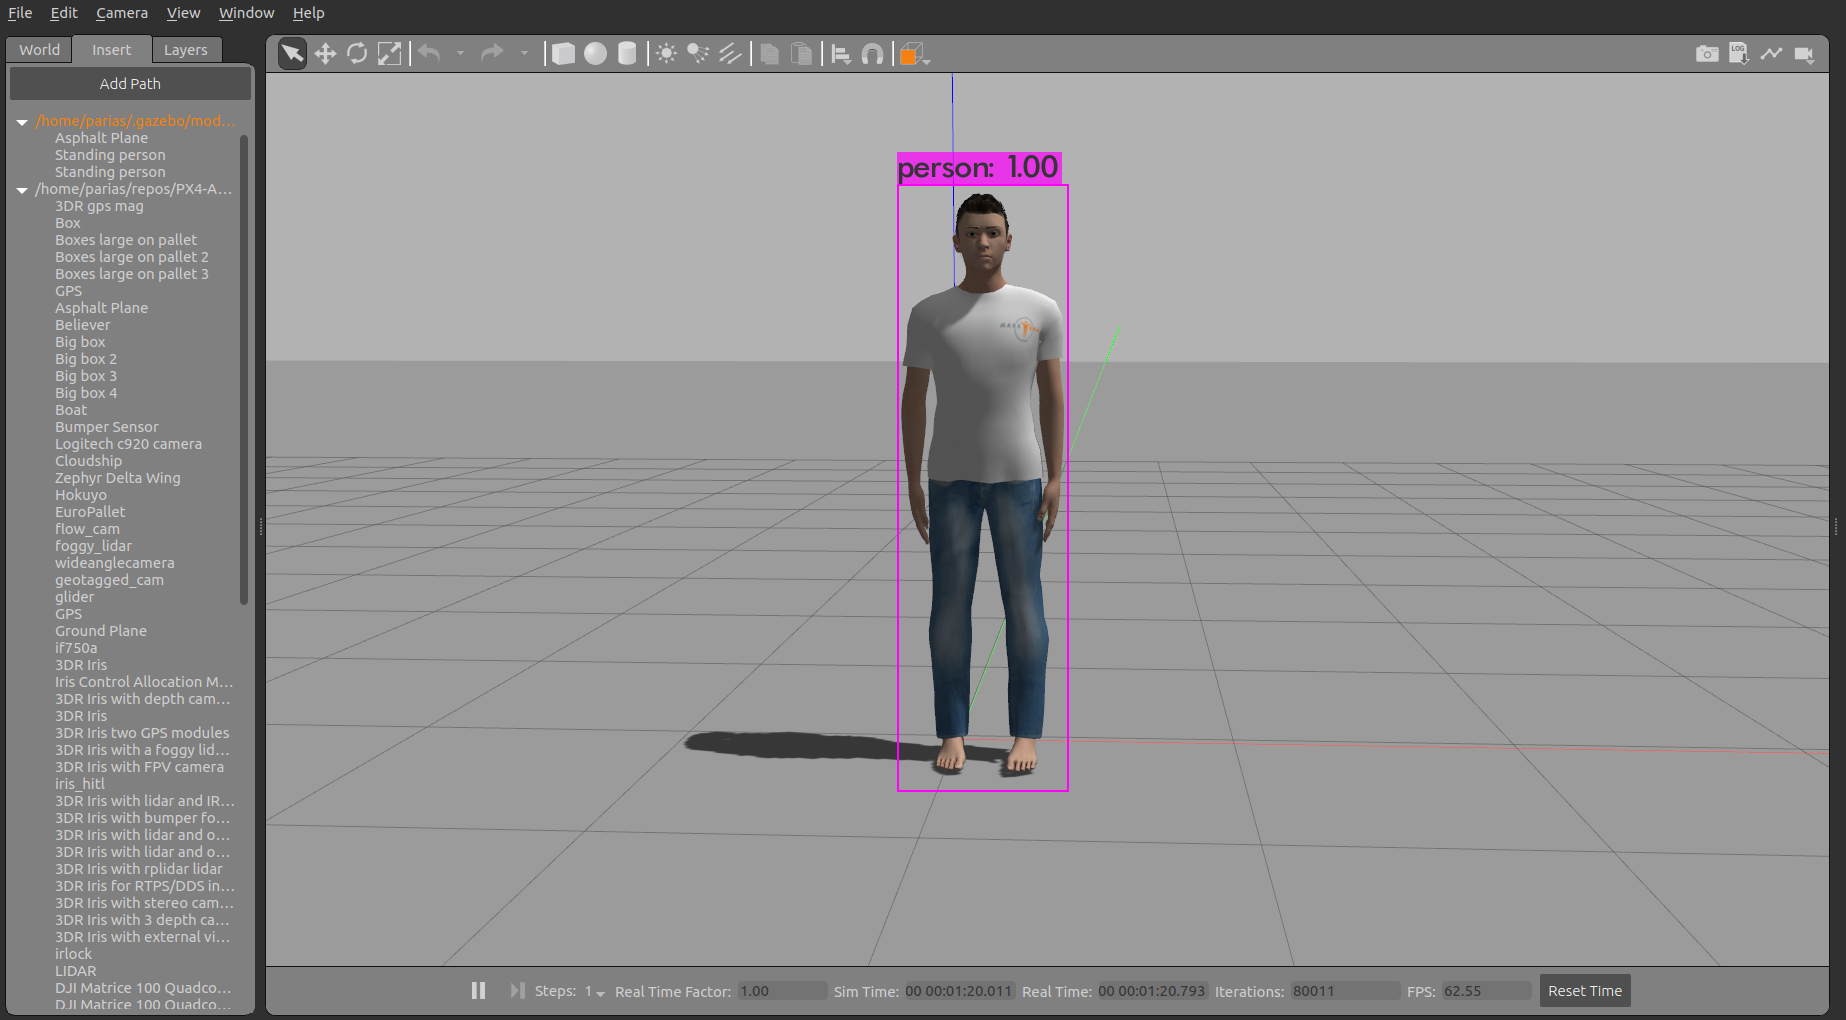
\includegraphics[width=1\linewidth]{05/detected-person.png}
        \caption{Detección en simulación.}
    \end{subfigure}
        
    \begin{subfigure}[b]{0.7\textwidth}
        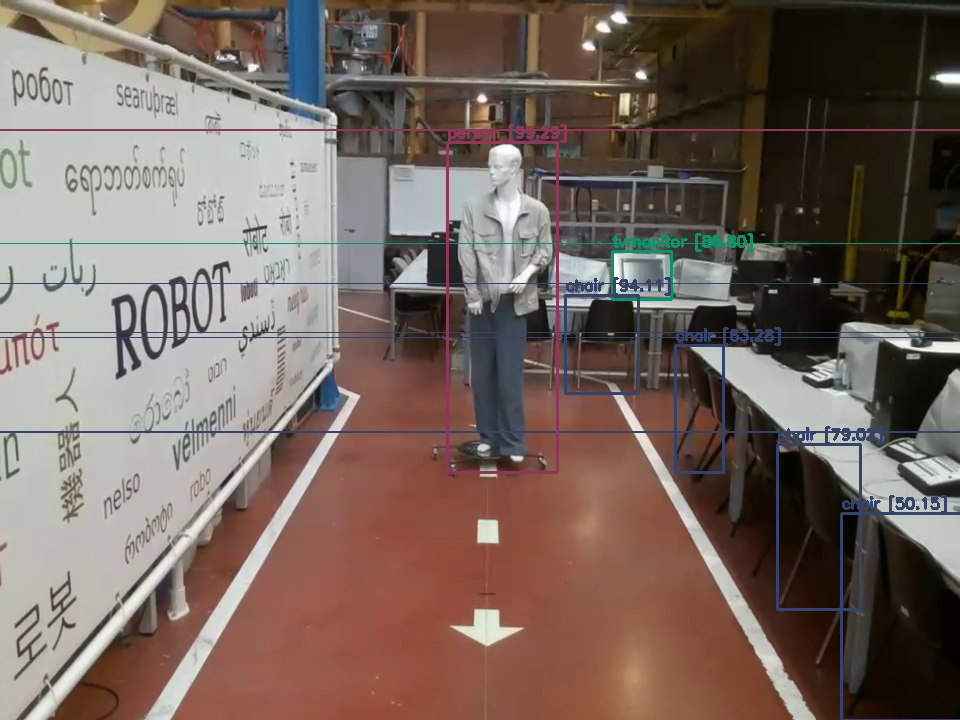
\includegraphics[width=1\linewidth]{05/detected-man.png}
        \caption{Detección de un maniquí con el \emph{tello}.}
    \end{subfigure}
    
    \caption{Detecciones en la aplicación \emph{sigue-persona}.}
    \label{fig:fp-det}
\end{figure}

La identificación se realiza almacenando posiciones anteriores de una detección considerada como ``principal''. La selección de la detección principal depende del número de detecciones. Partiendo de una situación donde no exista detección principal, si el número de personas detectadas es nulo, no existe objeto sobre el que realizar el seguimiento. En caso de que solo una persona sea detectada, es seleccionada como principal, y en caso de que haya más de una detección, la persona con confianza más alta es elegida como principal. \\
Sobre la detección principal se almacenan las posiciones de los últimos centroides sobre la imagen en una cola FIFO (\emph{First-In-First-Out}, último en entrar primero en salir) finita. La longitud de la cola es 5, lo que indica que se guardan las últimas cinco posiciones de la identificación. Sobre las nuevas detecciones se calculan sus centroides y se comparan con la media de los centroides almacenados en la cola. La detección con el centroide más próximo, es considerado como el objeto a seguir. La Figura \ref{fig:esq-ident} muestra el esqueda de la cola de identificación

\begin{figure}[!ht]
 	\ffigbox[\FBwidth] {
 	    \caption[Esquema de identificación en \emph{sigue-persona}]{Esquema de identificación en \emph{sigue-persona}.}
        \label{fig:esq-ident}
    }
 	{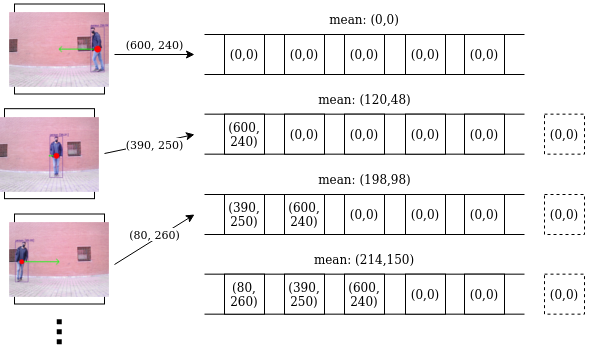
\includegraphics[width=0.8\textwidth]{05/fifo.png}}
\end{figure}

El bloque de percepción tiene por tanto una única salida, la persona detectada a seguir, si es que esta existe. En caso de no existir, la aeronave realizará un algoritmo de búsqueda consistente en dar vueltas sobre sí mismo hasta encontrar a una persona a la cual seguir.

Destacar que pese a que la percepción se centre en la detección de personas, la aplicación es fácilmente trasladable al seguimiento de otros objetos que pueda detectar la red, véase ``caballos'' o ``coches'' por ejemplo. Además, se ha elegido la red YOLOv4, pero en cualquier caso la detección se podría realizar con cualquiera otra red, con un coste de integración sencillo en la infraestructura.

\subsection*{Control}
El bloque de control es prácticamente idéntico, tal como se ha comentado durante la sección de diseño. La entrada del bloque es única, la persona detectada por el bloque de percepción. Sobre la caja delimitadora de la detección se calculan ciertas características que permiten calcular los errores a corregir por los controladores con sus salidas, las nuevas órdenes de velocidad de la aeronave. La Figura \ref{fig:esq-control-sp} recoge el esquema del bloque de control.

\begin{figure}[!ht]
 	\ffigbox[\FBwidth] {
 	    \caption[Esquema de control en \emph{sigue-persona}]{Esquema de control en \emph{sigue-persona}.}
        \label{fig:esq-control-sp}
    }
 	{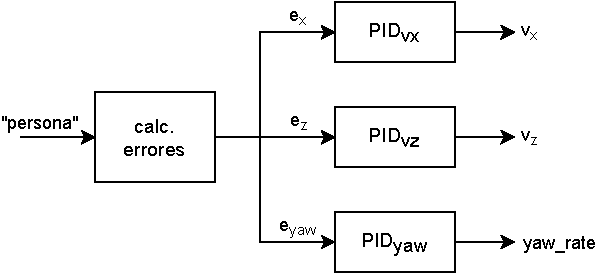
\includegraphics[width=0.65\textwidth]{05/fp-control.pdf}}
\end{figure}

Los controladores usados vuelven a ser tres PIDs, control en avance (\lstinline{vx}), control en altura (\lstinline{vz}) y control en guiñada (\lstinline{yaw_rate}). Los controles en altura y en guiñada son idénticos, mientras que el control en avance el ligeramente diferente. 

\begin{align}
    e_x = & \frac{area_{total}}{area_{det}} - \frac{area_{total}}{area_{target}} \label{eq:ex2} \\
    e_z = & c_y - obj_y \label{eq:ez2} \\
    e_{yaw} = & c_x - obj_x \label{eq:eyaw2}
\end{align}

Sobre la caja delimitadora de la persona se calcula el centroide. La posición del centroide se utiliza junto a la posición del centro de la imagen para calcular el error en altura y en guiñada (Ec. \ref{eq:ez2} y Ec. \ref{eq:eyaw2}). El error en avance (Ec. \ref{eq:ex2}) se calcula con la diferencia entre la relación de dos áreas. Por un lado, el área total y el área del objeto detectado, y por otro lado, el área total y un área de referencia. La relación de este segundo elemento tiene un valor de veinte ($\frac{area_{total}}{area_{target}} = 20$). Así pues, el control asegura que la persona detectada se encuentre aproximadamente a una distancia la cual el área de la persona ocupe una vigésima parte de la imagen, valor que experimentalmente se ha considerado aceptable. \\
La red es robusta frente a la orientación relativa entre la cámara y la persona (vista de perfil, desde atrás, etc.) y a la posición de la persona a detectar (de pie, sentado, agachado, etc.). Además, la red responde también correctamente frente a detecciones parciales por oclusiones o problemas similares. Utilizar el área de la detección como control de avance, ofrece un buen resultado en estos casos como se mostrará en la siguiente sección.

\begin{figure}[!ht]
 	\ffigbox[\FBwidth] {
 	    \caption{Respuesta del bloque de control en \emph{sigue-persona}.}
        \label{fig:sp-resp}
    }
 	{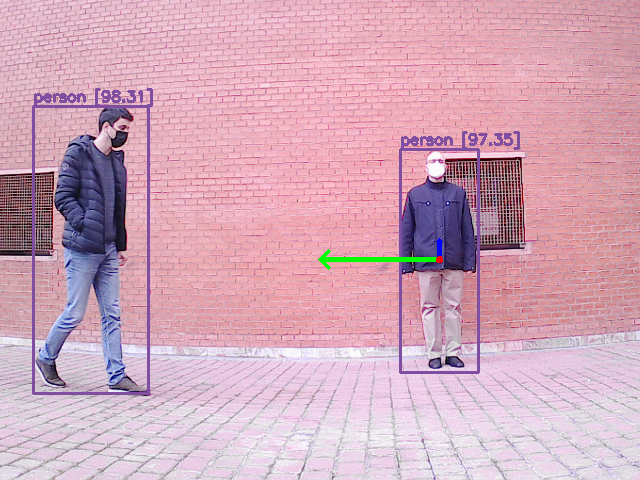
\includegraphics[width=0.75\textwidth]{05/fp-response.png}}
\end{figure}

La Figura \ref{fig:sp-resp} muestra la respuesta dada por el bloque de control a una entrada con varias detecciones. Las flechas indican la dirección que tomará el dron para corregir el error existente.

El constantes de los controladores PID no varían, pues las aeronaves son las mismas (ver Tabla \ref{tab:pid}). En el caso del PX4 utilizado en solo esta aplicación, no se han podido calcular los parámetros, ya que la aeronave ha tenido varios problemas prácticos que han impedido su vuelo. En la siguiente sección, se explicarán las dificultades encontradas con este dron.

\subsection*{Resultados}
Los resultados obtenidos se presentan de forma similar a la aplicación anterior, a través de distintas pruebas o experimentos. Se ha partido de un caso sencillo en simulado, y tras superarlo, se probó un nuevo caso con alguna dificultad añadida, hasta considerar que la aplicación es lo suficientemente robusta para probarla sobre una aeronave real. \\
Las pruebas en aeronave real se realizan en primer lugar sobre el Tello al ser una aeronave de menor tamaño y que se puede volar en interiores. Tras superar las pruebas sobre el dron de menor tamaño, se realizaron los experimentos sobre la aeronave de mayor tamaño, el PX4 propio. Así pues, la aplicación se ha probado sobre las tres plataformas disponibles.

Sin embargo, debido a diversos problemas con la aeronave, no se han podido realizar vuelos con la misma, limitándose los experimentos a la parte de percepción con el procesado a bordo de la aeronave con PX4. \\
El principal problema detectado es una carencia en la potencia de alimentación del dispositivo embebido a bordo de la aeronave. La batería abordo no es capaz de alimentar con suficiente potencia al dron y a la NVIDIA Jetson al mismo tiempo, cuando esta segunda está ejecutando tareas con grandes prestaciones como requiere la red neuronal. \\
Además, a lo largo del desarrollo se han detectado otros errores que sí se han podido subsanar. Es el caso de la actualización del NVIDIA JetPack al último disponible, necesario para poder ejecutar la red neuronal a bordo, la instalación de una antena WiFi para las comunicaciones o el reemplazo del sensor GPS y de uno de los motores, los cuales se encontraban dañados.

Pese a no conseguir volar dicha aeronave, se presentan también los resultados obtenidos con esta, ya que se considera relevante para este trabajo embarcar en una aeronave todo el software desarrollado. Esto es debido a que en aeronaves con el procesamiento en el segmento tierra, como es el caso del Tello, existen grandes limitaciones en la comunicación. Limitaciones tan importantes como la distancia o la degradación de la señal que hacen impracticable el experimento fuera de un entorno controlado.
% 

\begin{figure}[!ht]
 	\ffigbox[\FBwidth] {
 	    \caption{Experimento \emph{sigue-persona} con modelo estático.}
        \label{fig:sp-static}
    }
 	{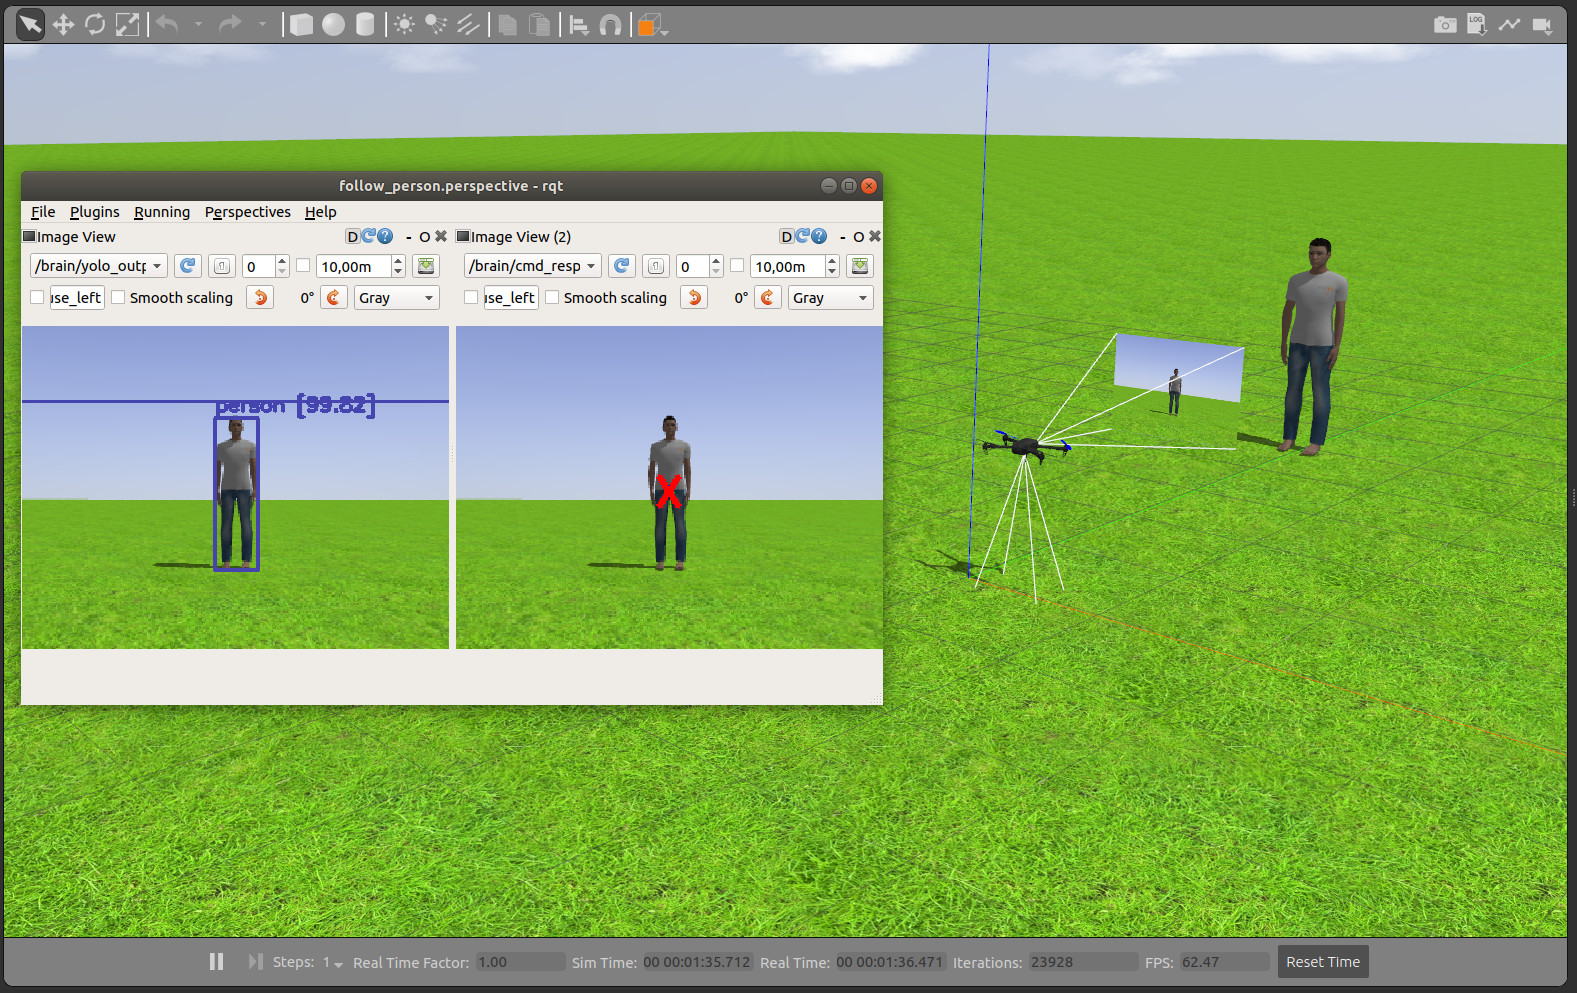
\includegraphics[width=0.95\textwidth]{05/static-fp.jpg}}
\end{figure}

Los experimentos se han iniciado en simulado, partiendo de un experimento simple con la persona a seguir estática (ver Fig. \ref{fig:sp-static}). En segundo lugar, se ha dotado de movimiento al modelo, probando la aplicación en un caso ya más cercano al mundo y también más complejo. Finalmente, se ha probado la aplicación sobre un entorno con varios modelos de personas, moviendo indistintamente los modelos a placer (Fig. \ref{fig:sp-multi}).

\begin{figure}[!ht]
 	\ffigbox[\FBwidth] {
 	    \caption{Experimento \emph{sigue-persona} con múltiples modelos.}
        \label{fig:sp-multi}
    }
 	{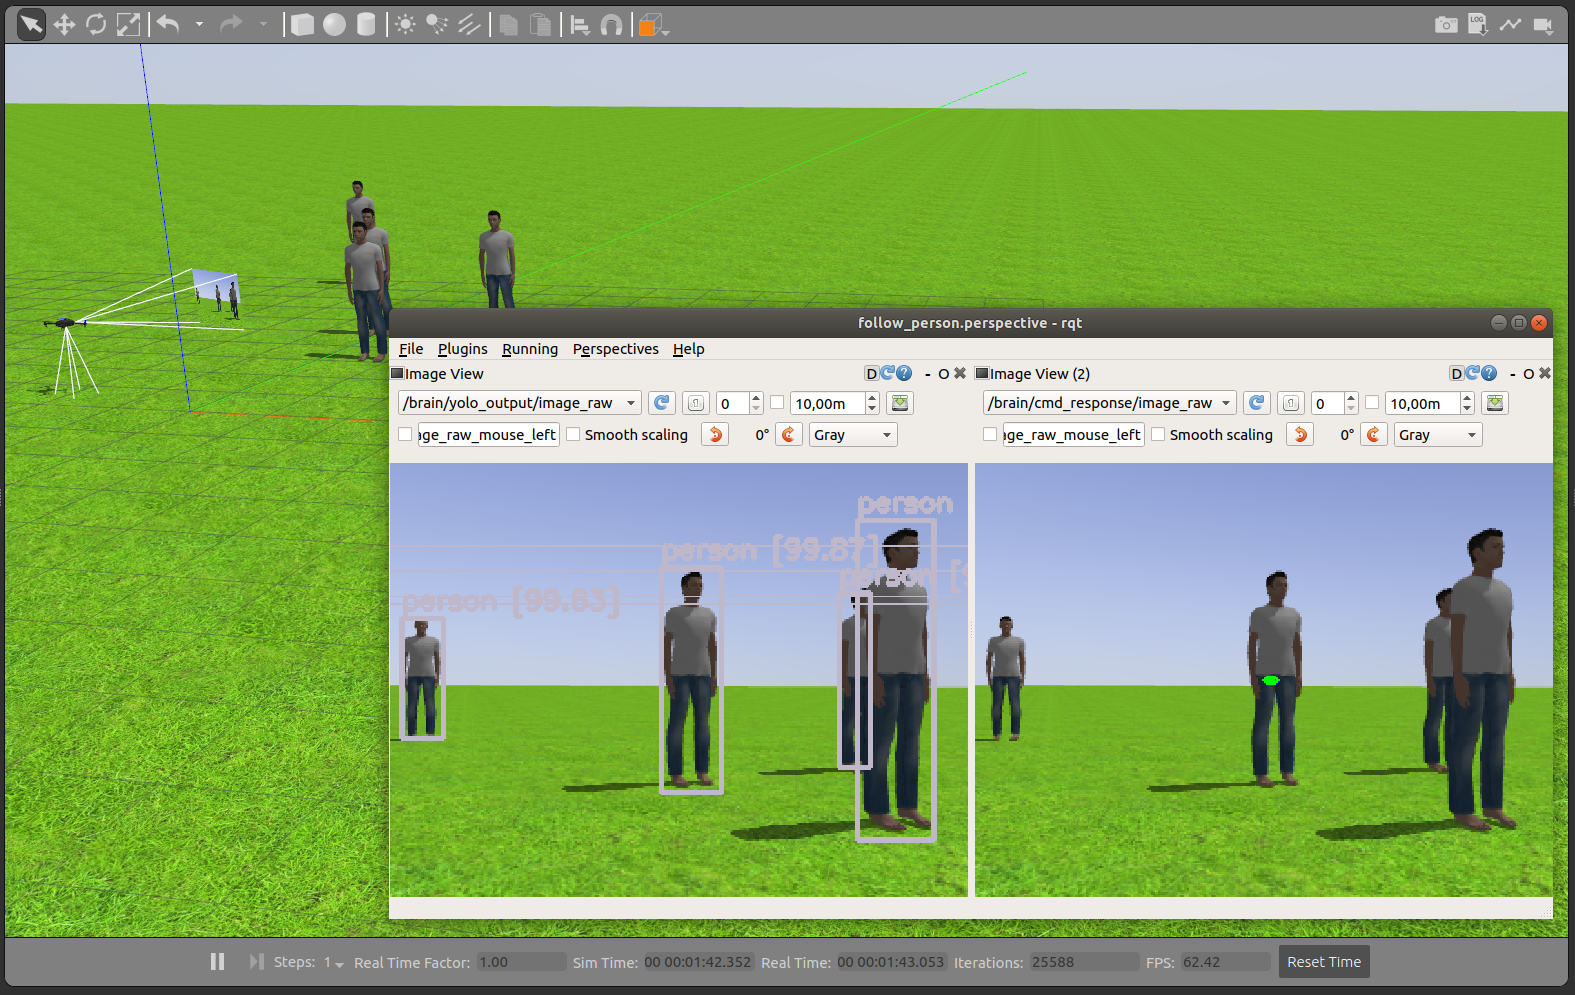
\includegraphics[width=0.95\textwidth]{05/multi.png}}
\end{figure}

\newpage
Tras superar con éxito estas primeras pruebas en simulado, la aplicación se ha probado con la primera de las aeronaves reales, el Tello. De forma similar, se ha partido de un caso sencillo, con una única persona estática, en este caso un maniquí. A continuación, el maniquí se ha substituidos por una persona, capaz de moverse en los distintos ejes de control, donde se ha observado un funcionamiento correcto del seguimiento. Recalcar que los experimentos realizados con el Tello se han realizado en interiores, donde el uso tradicional de los drones, por posición GPS, no es posible. La Figura \ref{fig:pasillo} recoge uno de los experimentos realizados, donde el dron Tello sigue a una persona a través de un pasillo.

\begin{figure}[htp]
    \ffigbox[\FBwidth]
    {\caption{Cruce trasero de persona.} \label{fig:back_ocl}}
 	{\includegraphics[width=.3\textwidth]{05/back_oclusion/0.png}\hfill
    \includegraphics[width=.3\textwidth]{05/back_oclusion/1.png}\hfill
    \includegraphics[width=.3\textwidth]{05/back_oclusion/2.png}}
\end{figure}

\begin{figure}[htp]
    \ffigbox[\FBwidth]
    {\caption{Cruce frontal de persona.} \label{fig:front_ocl}}
 	{\includegraphics[width=.3\textwidth]{05/front_oclusion/0.png}\hfill
    \includegraphics[width=.3\textwidth]{05/front_oclusion/1.png}\hfill
    \includegraphics[width=.3\textwidth]{05/front_oclusion/2.png}}
\end{figure}

Finalmente, la aplicación se ha probado en exteriores con la aeronave de mayor tamaño. Pese a su gran limitación de no poder volar, se ha comprobado el correcto funcionamiento del bloque de percepción con el procesamiento a bordo de la aeronave. Entre los experimentos realizados, se ha probado el funcionamiento de la aplicación frente a oclusiones entre varias personas. Los experimentos han sido dos, uno donde el cruce de la persona es por detrás del elemento a seguir (ver Fig. \ref{fig:back_ocl}) y otro más complejo donde el cruce se realiza por delante de la persona sobre la que se realiza el seguimiento (ver Fig. \ref{fig:front_ocl}. En este segundo caso, se puede observar como la detección se pierde cuando la persona identificada como a seguir está oculto sobre la segunda persona que cruza. Sin embargo, la identificación  permite mantener el seguimiento a la persona correcta cuando esta vuelve a ser detectada.

Las pruebas realizadas con aeronaves reales han sido diversas y de distinta dificultad. Los experimentos han sido numerosos, no solo se ha dotado de movimiento al objeto a seguir, sino que se ha probado con diferentes personas y posiciones de las mismas, número de personas en la imagen, iluminaciones y entornos. La Figura \ref{fig:mosaico} recoge ejemplos de las distintas circunstancias probadas.

Los diferentes experimentos se han recogido en varios vídeos disponibles para su visualización en una lista de reproducción\footnote{\url{https://youtube.com/playlist?list=PL2ebURGAzRwtsXui0GPFuQsIBJotnTIXj}} que recopila todas las pruebas realizada (ver figura \ref{fig:yt-fp}).

\begin{figure}[!ht]
 	\ffigbox[\FBwidth] {
 	    \caption{Lista de reproducción \emph{sigue-persona}.}
        \label{fig:yt-fp}
    }
 	{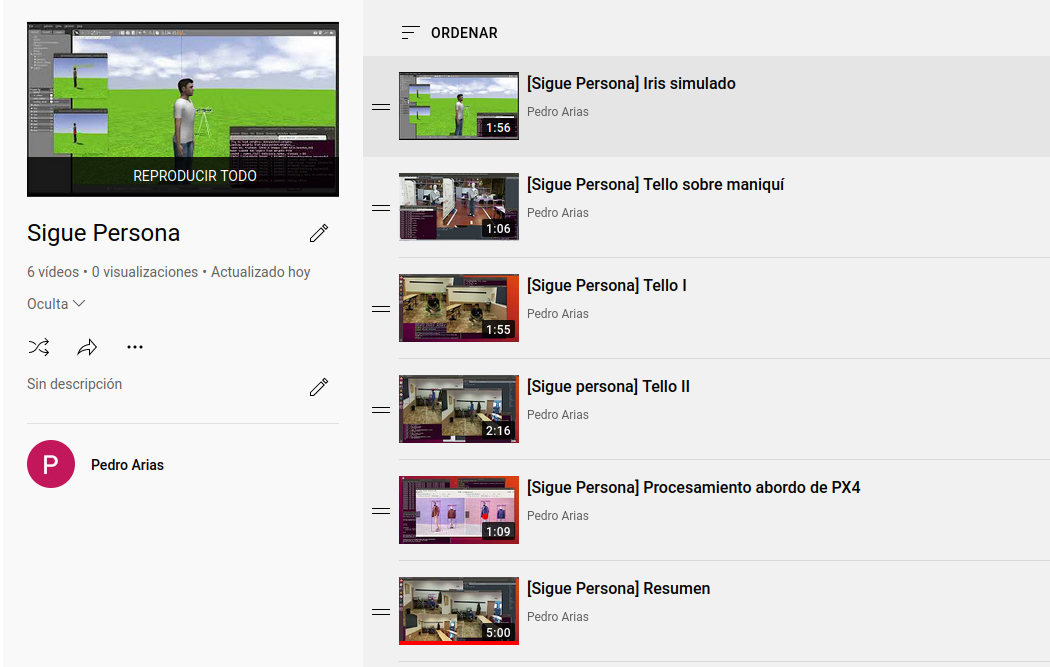
\includegraphics[width=0.9\textwidth]{05/yt-sigue-pers.png}}
\end{figure}

\begin{figure}[htp]
    \caption{Seguimiento de una persona por un pasillo.} \label{fig:pasillo}
 	\includegraphics[width=0.9\textwidth]{05/pasillo/1.png} \\
    \includegraphics[width=0.9\textwidth]{05/pasillo/2.png} \\
    \includegraphics[width=0.9\textwidth]{05/pasillo/4.png} \\
    \includegraphics[width=0.9\textwidth]{05/pasillo/5.png}
\end{figure}

\begin{figure}[htp]
    \caption{Ejemplos de la aplicación \emph{sigue-persona} bajo diferentes circunstancias.} \label{fig:mosaico}
 	\includegraphics[width=.33\textwidth]{05/mosaico/0.png}\hfill
    \includegraphics[width=.33\textwidth]{05/mosaico/1.png}\hfill
    \includegraphics[width=.33\textwidth]{05/mosaico/2.png}
    
    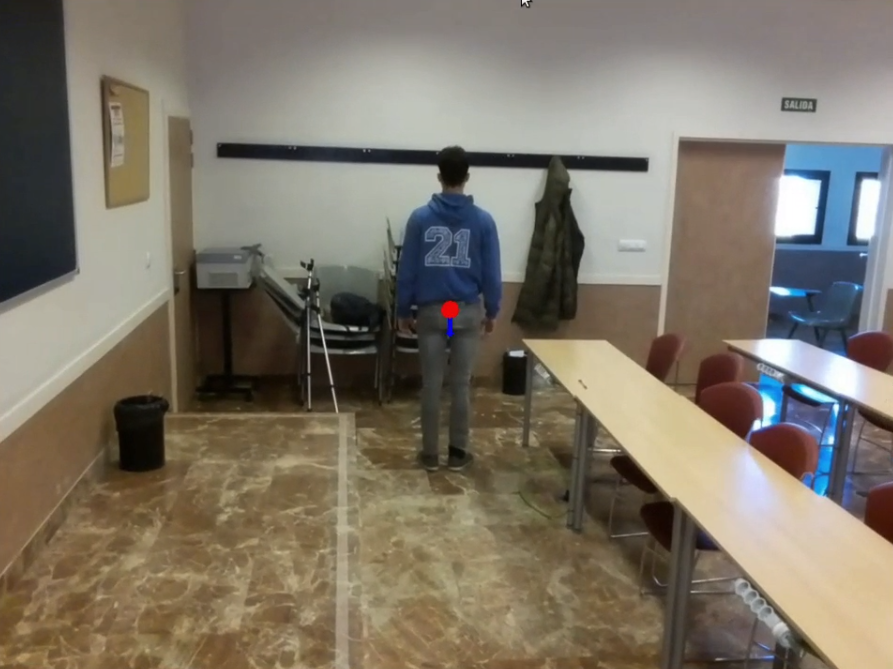
\includegraphics[width=.33\textwidth]{05/mosaico/3.png}\hfill
    \includegraphics[width=.33\textwidth]{05/mosaico/4.png}\hfill
    \includegraphics[width=.33\textwidth]{05/mosaico/5.png}
    
    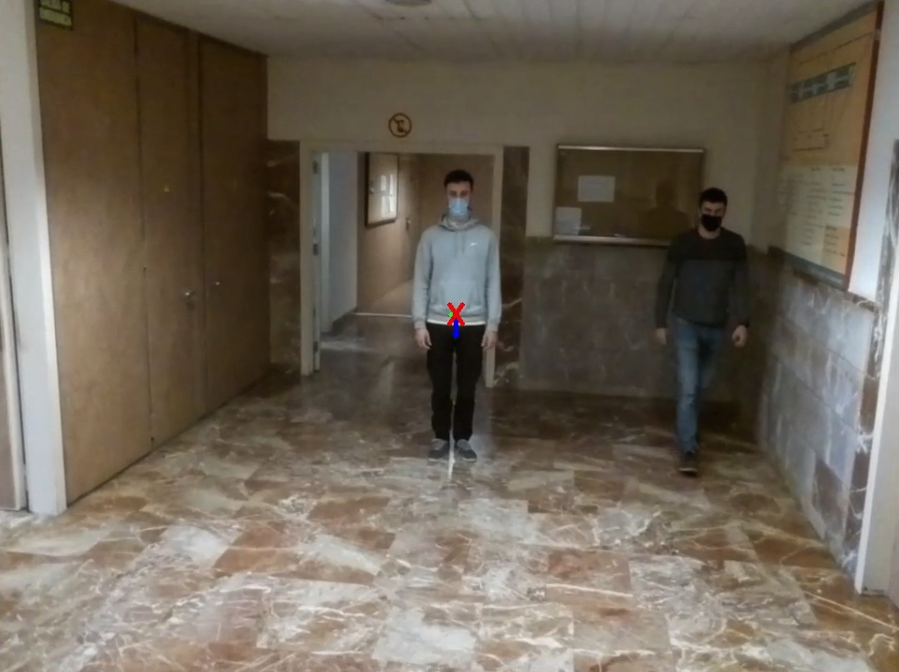
\includegraphics[width=.33\textwidth]{05/mosaico/6.png}\hfill
    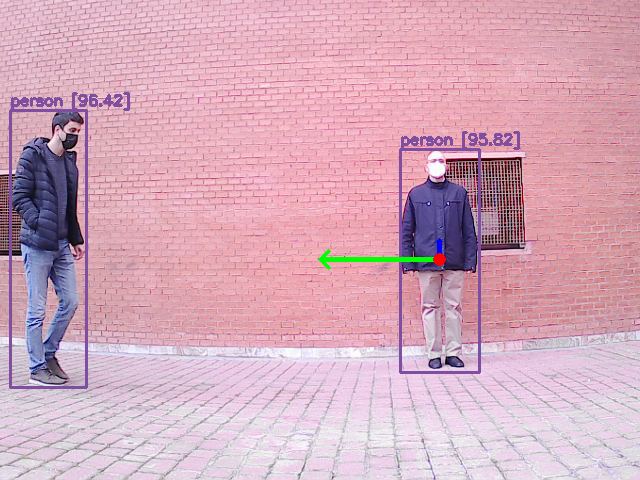
\includegraphics[width=.33\textwidth]{05/mosaico/7.png}\hfill
    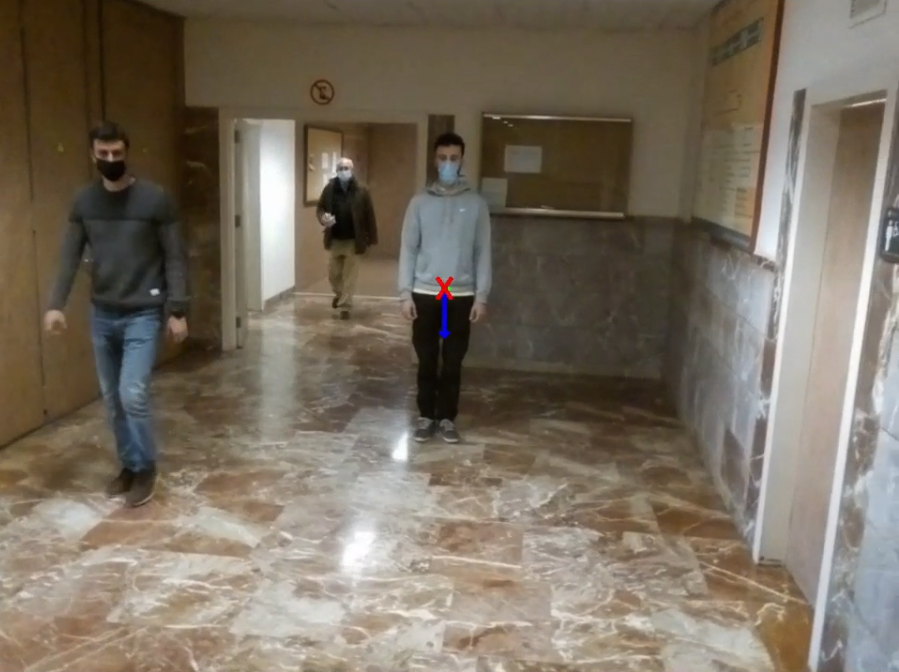
\includegraphics[width=.33\textwidth]{05/mosaico/8.png}
\end{figure}


\end{document}